% Appendix content consolidated

\chapter{Appendices}

\section{\texorpdfstring{\large\textbf{Mathematical Derivations}}{Mathematical Derivations}}

\subsection{Signal Model Derivations}
\label{app:signal_derivations}

This section provides detailed mathematical derivations for the signal models presented in Chapter 3. We begin with the fundamental signal model and derive the key expressions used throughout this thesis.

Consider the received signal at the secondary user, which can be expressed as:

\begin{equation}
r(t) = 
\begin{cases}
    n(t), & \text{H}_0 \\
    h_{ps}s(t) + n(t), & \text{H}_1 \\
    h_{ms}s'(t) + n(t), & \text{H}_2
\end{cases}
\end{equation}

where $h_{ps}$ and $h_{ms}$ are the channel gains from primary user and malicious user to secondary user, respectively; $s(t)$ is the primary user signal; $s'(t)$ is the emulated signal; and $n(t)$ is the additive white Gaussian noise.

The log-normal shadowing model used to characterize the wireless channel can be derived as follows. The path loss in dB at distance $d$ is given by:

\begin{equation}
    PL(d) = PL(d_0) + 10\alpha\log_{10}\left(\frac{d}{d_0}\right) + X_\sigma
\end{equation}

where $PL(d_0)$ is the path loss at the reference distance $d_0$, $\alpha$ is the path loss exponent, and $X_\sigma$ is a zero-mean Gaussian random variable with standard deviation $\sigma$.

The channel gain can be derived from the path loss as:

\begin{equation}
    h = 10^{-PL(d)/20} = 10^{-PL(d_0)/20} \cdot 10^{-\alpha\log_{10}(d/d_0)/2} \cdot 10^{-X_\sigma/20}
\end{equation}

Simplifying:

\begin{equation}
    h = K \cdot \left(\frac{d}{d_0}\right)^{-\alpha/2} \cdot 10^{-X_\sigma/20}
\end{equation}

where $K = 10^{-PL(d_0)/20}$ is a constant.

\subsection{Feature Extraction Mathematics}
\label{app:feature_math}

This section provides detailed mathematical expressions for the feature extraction methods described in Chapter 4.

\subsubsection{Statistical Moments}

For a set of RSS measurements $\{r_1, r_2, \ldots, r_N\}$ from $N$ secondary users, the statistical moments are calculated as follows:

\begin{equation}
    \mu = \frac{1}{N}\sum_{i=1}^{N} r_i
\end{equation}

\begin{equation}
    \sigma^2 = \frac{1}{N}\sum_{i=1}^{N} (r_i - \mu)^2
\end{equation}

\begin{equation}
    \gamma = \frac{1}{N\sigma^3}\sum_{i=1}^{N} (r_i - \mu)^3
\end{equation}

\begin{equation}
    \kappa = \frac{1}{N\sigma^4}\sum_{i=1}^{N} (r_i - \mu)^4 - 3
\end{equation}

\section{Algorithm Implementations}

\subsection{DBSCAN Algorithm}
\label{app:dbscan}

The DBSCAN algorithm implementation used in this thesis is presented below:

\begin{algorithm}[H]
\caption{\textbf{DBSCAN Clustering for PUEA Detection}}
\label{alg:dbscan}
\begin{algorithmic}[1]
\Require{RSS feature matrix $X$, distance threshold $\epsilon$, minimum points MinPts}
\Ensure{Cluster assignments for each time slot}

\Function{DBSCAN}{$X$, $\epsilon$, MinPts}
    \State C $\gets$ 0 \Comment{Initialize cluster counter}
    \State $\text{labels} \gets \{\text{UNCLASSIFIED for all points in X}\}$
    
    \For{each point $p$ in $X$}
        \If{$\text{labels}[p] \neq \text{UNCLASSIFIED}$}
            \State \textbf{continue}
        \EndIf
        
        \State $\text{Neighbors} \gets \text{regionQuery}(X, p, \epsilon)$
        
        \If{$|\text{Neighbors}| < \text{MinPts}$}
            \State $\text{labels}[p] \gets \text{NOISE}$
        \Else
            \State C $\gets$ C + 1
            \State $\text{expandCluster}(X, p, \text{Neighbors}, C, \epsilon, \text{MinPts})$
        \EndIf
    \EndFor
    
    \State \Return labels
\EndFunction

\Function{expandCluster}{$X$, $p$, $\text{Neighbors}$, $C$, $\epsilon$, $\text{MinPts}$}
    \State $\text{labels}[p] \gets C$
    
    \For{each point $q$ in $\text{Neighbors}$}
        \If{$\text{labels}[q] = \text{UNCLASSIFIED}$}
            \State $\text{labels}[q] \gets C$
            
            \State $\text{NeighborsQ} \gets \text{regionQuery}(X, q, \epsilon)$
            
            \If{$|\text{NeighborsQ}| \geq \text{MinPts}$}
                \State $\text{Neighbors} \gets \text{Neighbors} \cup \text{NeighborsQ}$
            \EndIf
        \EndIf
    \EndFor
\EndFunction

\Function{regionQuery}{$X$, $p$, $\epsilon$}
    \State \Return $\{q \in X : \text{distance}(p, q) \leq \epsilon\}$
\EndFunction
\end{algorithmic}
\end{algorithm}

\subsection{Enhanced Detection with KNN}
\label{app:knn}

The pseudocode for the enhanced detection approach using KNN is as follows:

\begin{algorithm}[H]
\caption{\textbf{Enhanced Detection with KNN}}
\label{alg:enhanced_knn}
\begin{algorithmic}[1]
\Require{RSS feature matrix $X$, cluster assignments $C$, number of neighbors $k$}
\Ensure{Refined classification labels}

\Function{EnhancedKNN}{$X$, $C$, $k$}
    \State $\text{labels} \gets C$ \Comment{Initialize with clustering results}
    \State $\text{clusters} \gets \{\text{unique values in } C\}$
    \State $\text{means} \gets \{\text{mean of points in each cluster}\}$
    
    \For{each point $p$ in $X$}
        \State $\text{origCluster} \gets C[p]$
        \State $\text{knn} \gets \text{findKNearestNeighbors}(X, p, k)$
        
        \State $\text{clusterCounts} \gets \{0 \text{ for all clusters}\}$
        
        \For{each neighbor $n$ in $\text{knn}$}
            \State $\text{clusterCounts}[C[n]] \gets \text{clusterCounts}[C[n]] + 1$
        \EndFor
        
        \State $\text{majorityCluster} \gets \text{argmax}(\text{clusterCounts})$
        
        \If{$\text{majorityCluster} \neq \text{origCluster}$}
            \State $\text{confidence} \gets \text{clusterCounts}[\text{majorityCluster}] / k$
            
            \If{$\text{confidence} > \text{threshold}$}
                \State $\text{labels}[p] \gets \text{majorityCluster}$
            \EndIf
        \EndIf
    \EndFor
    
    \State \Return labels
\EndFunction
\end{algorithmic}
\end{algorithm}

\section{Experimental Data Samples}
\label{app:data}

Table \ref{tab:sample_data} presents a sample of the RSS measurements collected in the simulation environment for Scenario A, with path loss exponent $\alpha = 4$ and shadowing standard deviation $\sigma = 8$.

\begin{table}[htbp]
    \centering
    \caption{\textbf{Sample RSS measurements (dBm) at secondary users}}
    \label{tab:sample_data}
    \begin{tabular}{>{\centering\arraybackslash}c>{\centering\arraybackslash}c>{\centering\arraybackslash}c>{\centering\arraybackslash}c>{\centering\arraybackslash}c>{\centering\arraybackslash}c}
        \toprule
        \textbf{Time Slot} & \textbf{SU-1} & \textbf{SU-2} & \textbf{SU-3} & \textbf{$\cdots$} & \textbf{SU-30} \\
        \midrule
        1 (PU) & -72.3 & -68.9 & -81.5 & $\cdots$ & -76.8 \\
        2 (PU) & -71.9 & -69.3 & -80.2 & $\cdots$ & -77.1 \\
        3 (PUEA) & -58.4 & -63.7 & -60.8 & $\cdots$ & -65.3 \\
        4 (PU) & -73.5 & -67.8 & -82.1 & $\cdots$ & -75.9 \\
        5 (PUEA) & -57.9 & -62.8 & -61.3 & $\cdots$ & -64.7 \\
        $\vdots$ & $\vdots$ & $\vdots$ & $\vdots$ & $\ddots$ & $\vdots$ \\
        100 (PU) & -72.7 & -68.5 & -81.9 & $\cdots$ & -76.2 \\
        \bottomrule
    \end{tabular}
\end{table}

\section{Supplementary Results}
\label{app:results}

This section presents additional performance results that support the findings discussed in the main chapters but were omitted due to space constraints.

\subsection{Algorithm Performance under Extreme Shadowing}

Figure \ref{fig:extreme_shadowing} shows the detection performance under extreme shadowing conditions ($\sigma = 14$ dB).

\begin{figure}[htbp]
    \centering
    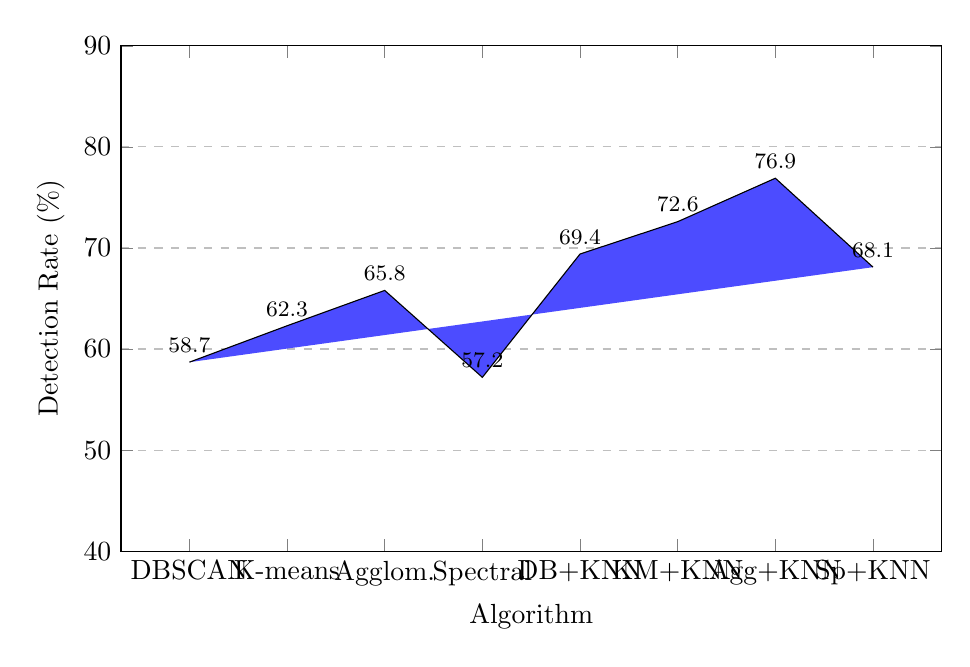
\begin{tikzpicture}
        \begin{axis}[
            width=12cm,
            height=8cm,
            ylabel={Detection Rate (\%)},
            xlabel={Algorithm},
            symbolic x coords={DBSCAN, K-means, Agglom., Spectral, DB+KNN, KM+KNN, Agg+KNN, Sp+KNN},
            xtick=data,
            ymin=40, ymax=90,
            ymajorgrids=true,
            grid style=dashed,
            nodes near coords,
            every node near coord/.append style={font=\footnotesize},
            ylabel near ticks,
            legend style={at={(0.5,1.05)}, anchor=south, legend columns=2},
            ]
            
            \addplot[fill=blue!70, draw=black] coordinates {
                (DBSCAN, 58.7)
                (K-means, 62.3)
                (Agglom., 65.8)
                (Spectral, 57.2)
                (DB+KNN, 69.4)
                (KM+KNN, 72.6)
                (Agg+KNN, 76.9)
                (Sp+KNN, 68.1)
            };
            
        \end{axis}
    \end{tikzpicture}
    \caption{Detection performance under extreme shadowing conditions}
    \label{fig:extreme_shadowing}
\end{figure}

\subsection{Computational Performance Comparison}

Table \ref{tab:computation_time} presents the average computation time required for each algorithm to process 100 time slots on the test hardware.

\begin{table}[htbp]
    \centering
    \caption{Average computation time for different algorithms (ms)}
    \label{tab:computation_time}
    \begin{tabular}{lcccc}
        \toprule
        \textbf{Algorithm} & \textbf{Scenario A} & \textbf{Scenario B} & \textbf{Scenario C} & \textbf{Average} \\
        \midrule
        DBSCAN & 65 & 64 & 66 & 65 \\
        K-means & 42 & 41 & 43 & 42 \\
        Agglomerative & 78 & 77 & 79 & 78 \\
        Spectral & 127 & 125 & 129 & 127 \\
        \midrule
        DBSCAN+KNN & 94 & 93 & 95 & 94 \\
        K-means+KNN & 67 & 66 & 68 & 67 \\
        Agglomerative+KNN & 112 & 111 & 113 & 112 \\
        Spectral+KNN & 162 & 160 & 164 & 162 \\
        \bottomrule
    \end{tabular}
\end{table}

\section{Symbol List}
\label{app:symbols}

Table \ref{tab:symbols} provides a comprehensive list of mathematical symbols used throughout this thesis.

\begin{table}[htbp]
    \centering
    \caption{List of mathematical symbols}
    \label{tab:symbols}
    \begin{tabular}{cl}
        \toprule
        \textbf{Symbol} & \textbf{Description} \\
        \midrule
        $\alpha$ & Path loss exponent \\
        $\sigma_{\psi}$ & Shadow fading standard deviation (dB) \\
        $d_{ij}$ & Distance between nodes $i$ and $j$ \\
        $P_t$ & Transmission power \\
        $P_r$ & Received power \\
        $\mu$ & Mean of RSS measurements \\
        $\sigma^2$ & Variance of RSS measurements \\
        $\gamma$ & Skewness of RSS distribution \\
        $\kappa$ & Kurtosis of RSS distribution \\
        $\epsilon$ & Distance threshold in DBSCAN \\
        $k$ & Number of neighbors in KNN \\
        $\delta$ & Refinement threshold for enhanced detection \\
        $C$ & Cluster assignments \\
        \bottomrule
    \end{tabular}
\end{table}
